\begin{enumerate}

	\item The digital circuit shown in Fig. \ref{fig:2004-gate-ee-68} generates a modified clockpulse at the output. Sketch the output waveform.
\label{prob:2004-gate-ee-68}
\hfill (GATE EE 2004)


\begin{figure}[h]
	\centering
	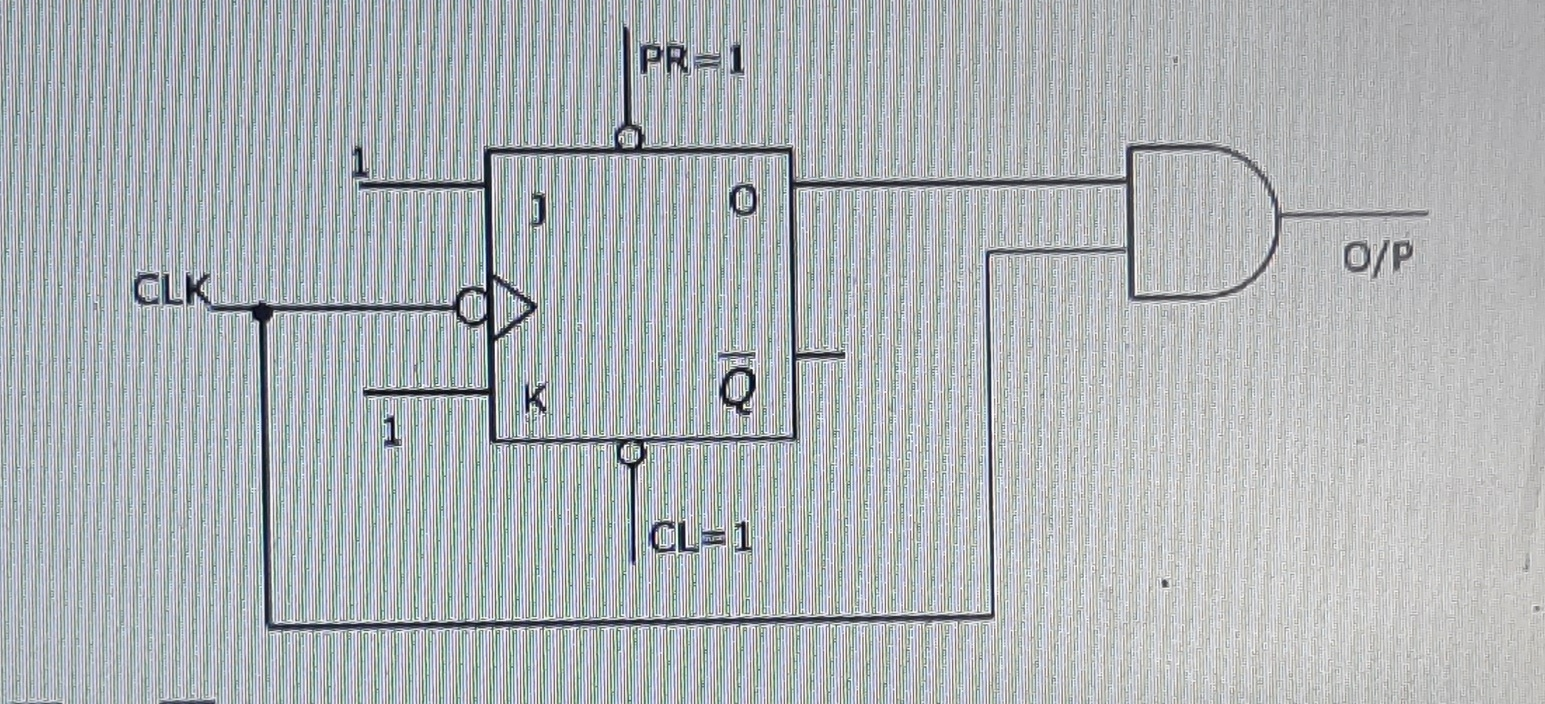
\includegraphics[width=\columnwidth]{figs/2004-gate-ee-68.jpg}
	\caption{}
\label{fig:2004-gate-ee-68}
\end{figure}
	\item 		
		A counter is constructed with three D flip-flops. The input-output pairs are named (D0, Q0), (D1, Q1), and (D2, Q2), where the subscript 0 denotes the least significant bit. The output sequence is desired to be the Gray-code sequence 000, 001, 011, 010, 110, 111, 101, and 100, repeating periodically. Note that the bits are listed in the Q2 Q1 Q0 format. Find the combinational logic expression for D1.
\label{prob:2021-gate-ee-37}
\hfill (CBSE 2021)

\end{enumerate}
